% !TEX encoding = UTF-8 Unicode
\documentclass{article}

\usepackage{polski}
\usepackage[utf8]{inputenc}
\usepackage{subfig}
\usepackage{tikz}

\usepackage[a4paper, left=2.5cm, right=2.5cm, top=3.5cm, bottom=3.5cm, headsep=1.2cm]{geometry}

\linespread{1.3}
 
\begin{document}

\begin{titlepage}
\centering
{\scshape\LARGE Politechnika Wrocławska \par}
{\scshape\Large Katedra Informatyki Technicznej\par}

	\vspace{1cm}
	{\scshape\Large Inżynieria Oprogramowania\par}
	\vspace{1.5cm}
	{\huge\bfseries Zapoznanie się z wybranym narzędziem UML - wprowadzenie do UML\par}
	\vspace{2cm}
	{\Large\itshape Magdalena Biernat\par}
	{\Large\itshape Mateusz Bortkiewicz\par}
	\vfill
	Opiekun\par
	prof. dr hab. inż. Jan Magott 

	\vfill
	{\large \today\par}
\end{titlepage}
\newpage
\section{Wprowadzenie}
Niniejsze sprawozdanie jest dokumentem z pierwszego laboratorium \textit{Inżynierii Oprogramowania}.
\subsection{Cel laboratorium}
Wprowadzenie do UML – wykonanie prostego projektu programu za pomocą
wybranych diagramów UML i implementacja projektu programu w języku
Java.
\subsection{Plan pracy}
Postawiono wykonać zadania wg instrukcji prowadzącego:
\begin{itemize}
\item Zapoznanie się z punktami 1 i 2 instrukcji laboratorium.
\item Wykonanie projektu UML w środowisku Visual Paradigm.
\item Odwzorowanie programu w języku Java w środowisku Eclipse.
\end{itemize}
\section{Laboratorium}
\subsection{Przepisanie}
\subsubsection{Projekt UML}
Na potrzeby zapoznania się z językiem UML, stworzono projekt na podstawie instrukcji. Widok na wszystkie diagramy stworzone w Visual Paradigm wygląda następująco:
\begin{figure}[h]
\centering
	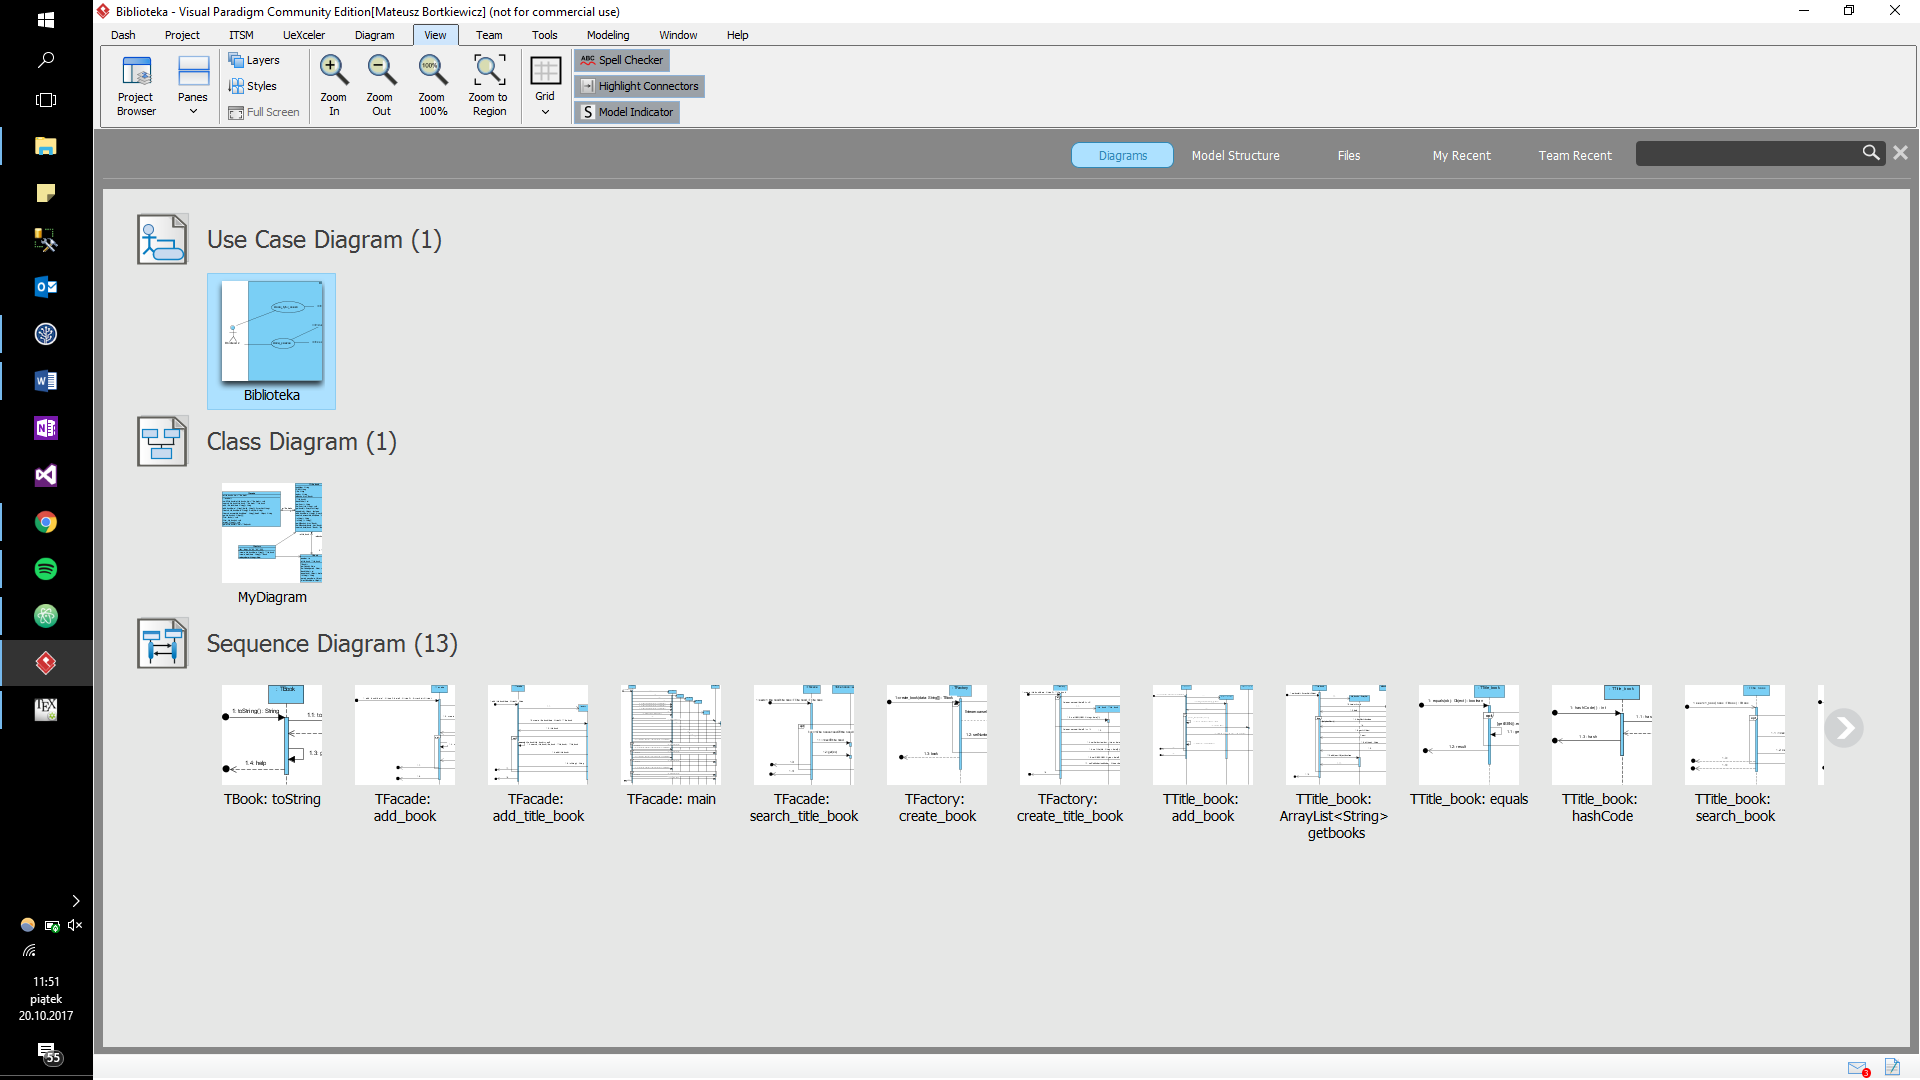
\includegraphics[width=15cm]{vp1.png}
	\caption{Stworzone diagramy}
	\label{fig:obrazek 1}
\end{figure}
\subsubsection{Odwzorowanie w Javie}
Kolejnym krokiem było odwzorowanie środowiska w języku Java. W celu efektywniejszego stworzenia projektu, porzucono rozwiązanie w środowisku NetBeans i wykonano projekt w środowisku Eclipse. W wyniku odwzorowania i skompilowania projektu, uzyskano odpowiedź w konsoli:
\begin{verbatim}
[Title: Title1 Author: Author1 ISBN: ISBN1 Publisher: Publisher1,
Title: Title2 Author: Author2 ISBN: ISBN2 Publisher: Publisher2,
Title: Title3 Author: Author3 ISBN: ISBN3 Publisher: Publisher3]
[Title: Title1 Author: Author1 ISBN: ISBN1 Publisher: Publisher1 Number: 1]
[Title: Title2 Author: Author2 ISBN: ISBN2 Publisher: Publisher2 Number: 1]
[Title: Title2 Author: Author2 ISBN: ISBN2 Publisher: Publisher2 Number: 1]
[Title: Title2 Author: Author2 ISBN: ISBN2 Publisher: Publisher2 Number: 2]
\end{verbatim}
Uzyskana odpowiedź jest zgodna z tą, która jest zawarta w instrukcji, a co za tym idzie: ćwiczenie zostało wykonane poprawnie.
\subsection{Część kreatywna}
Na potrzeby ćwiczenia stworzono klasę XLender, która odzwierciedla wypożyczającego. Klasa posiada pola tj. imię, nazwisko, PESEL, adres. W celu obsługi nowopowstałej klasy, dodano lub zmodyfikowano pola lub metody w klasach istniejących. I tak klasa TFacade otrzymała metody \textit{search\_lender(), add\_lender(), getLenders()} oraz pole \textit{lenders} klasy XLender. Metoda \textit{main()} została odpowiednio zmodyfikowana. Klasa TFactory otrzymała natomiast metodę \textit{create\_lender}.
\subsubsection{Project UML}
W diagramie klas dodano klasę XLender oraz zmodyfikowano odpowiednie klasy dodając im odpowiednie metody.
\begin{figure}[!ht]
\centering
	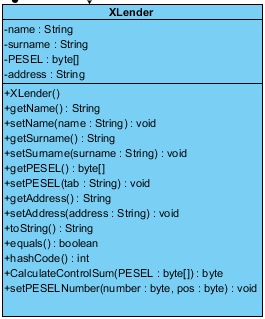
\includegraphics[width=5cm]{XLender.png}
	\caption{Stworzona klasa}
	\label{fig:obrazek 2}
\end{figure}
\newpage
W diagramach sekwencji dodano diagramy dla setera PESEL-u klasy XLender, add\_lender i search\_lender klasy TFacade, create\_lender klasy TFactory. Zmodyfikowano m.in metodę main w klasie TFacade.
\begin{figure}[!ht]
\centering
	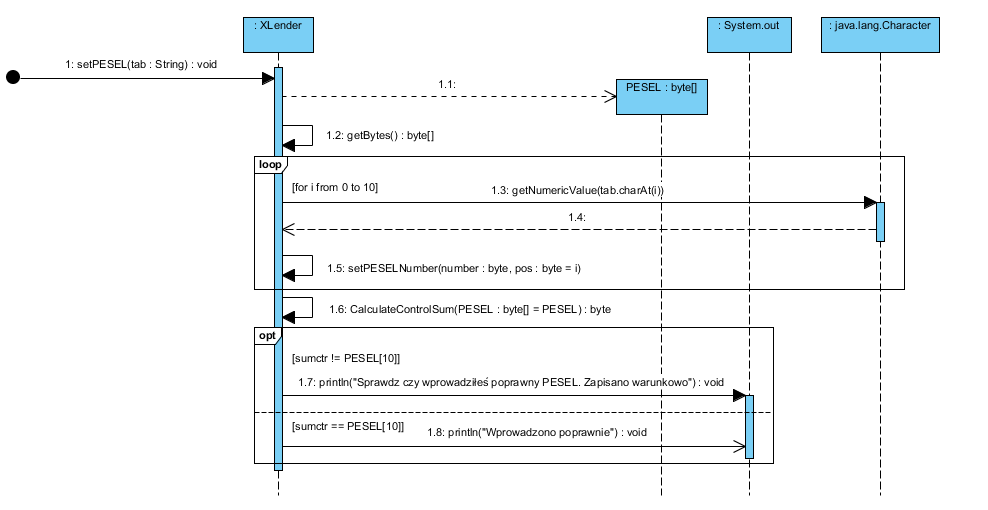
\includegraphics[width=12cm]{XLendersetPESEL.PNG}
	\caption{XLender: setPESEL}
	\label{fig:obrazek 3}
\end{figure}
\begin{figure}[!ht]
\centering
	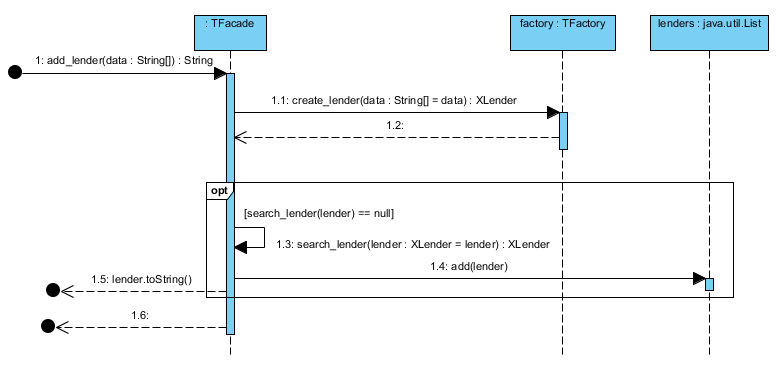
\includegraphics[width=12cm]{TFacadeadd_lender.PNG}
	\caption{TFacade: add\_lender}
	\label{fig:obrazek 4}
\end{figure}
\begin{figure}[!ht]
\centering
	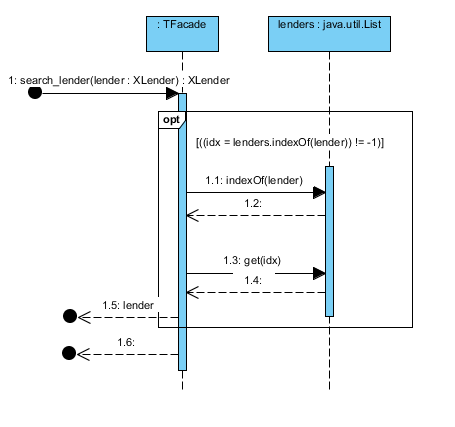
\includegraphics[width=8cm]{TFacadesearch_lender.PNG}
	\caption{TFacade: search\_lender}
	\label{fig:obrazek 5}
	\end{figure}
	\begin{figure}[!ht]
\centering
	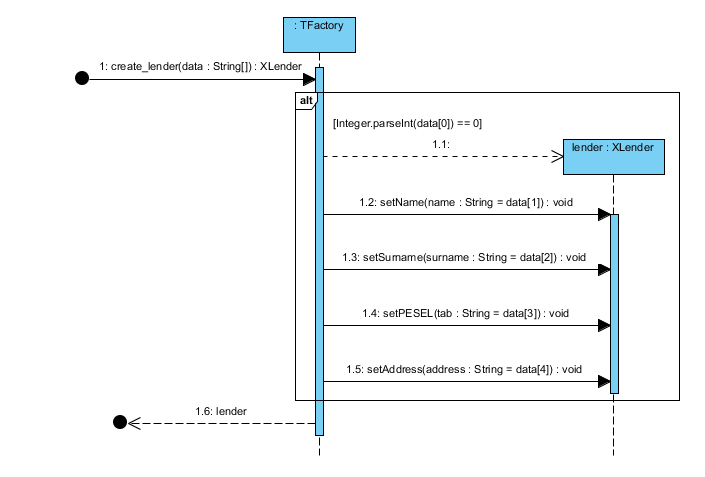
\includegraphics[width=12cm]{TFactorycreate_lender.PNG}
	\caption{TFactory: create\_lender}
	\label{fig:obrazek 6}
\end{figure}
\newpage
\subsubsection{Odzwierciedlenie w Javie}
Klasa XLender posiada pola:
\begin{verbatim}
	private String name;
	private String surname;
	private String address;
	private byte[] PESEL;
\end{verbatim}
oraz odpowiednie settery i gettery. Tutaj m.in. setter PESELU:
\begin{verbatim}
	public void setPESEL(String tab) {
		this.PESEL = new byte[11];

		for (byte i = 0; i < 11; i++)
			setPESELNumber((byte) Character.getNumericValue(tab.charAt(i)), i);

		byte sumctr = CalculateControlSum(this.PESEL);
		if (sumctr != this.PESEL[10])
			System.out.println("Sprawdz czy wprowadziłeś poprawny PESEL. Zapisano warunkowo");
		else
			System.out.println("Wprowadzono poprawnie");
	}
\end{verbatim}
W klasie TFacade mamy nowe metody:
\begin{verbatim}
	public XLender search_lender(XLender lender){
		
		int idx;
		if((idx = lenders.indexOf(lender)) != -1){
			lender = lenders.get(idx);
			return lender;
		}
		return null;
	}

	public String add_lender(String data[]){
		TFactory factory = new TFactory();
		XLender lender = factory.create_lender(data);
		if(search_lender(lender) == null){
			lenders.add(lender);
			return lender.toString();
		}
		return null;
	}
\end{verbatim}
Podobnie w klasie TFactory
\begin{verbatim}
	public XLender create_lender(String data[]){
		XLender lender = null;
		switch (Integer.parseInt(data[0])){
		case 0:
			lender = new XLender();
			lender.setName(data[1]);
			lender.setSurname(data[2]);
			lender.setPESEL(data[3]);
			lender.setAddress(data[4]);
			break;
		}
		return lender;
	}
\end{verbatim}
Pełen kod oraz diagramy znajdują się w załączonych plikach.
\end{document}